\chapter{Intent Change Estimation Based on Physical Interactions of an	Exoskeleton User}\label{chapter:BKF}
The IMM estimation framework presented previously is reactive as it monitors signs of gait transition i.e.~if the CoM trajectory after gait transition does not resemble library gaits, the IMM algorithm will misidentify the intended change until after it has been realized. However, anticipative intent inference is more desirable to time the assistance delivery appropriately and help the user realize their intended gait transition. Improper assistance timing may result in the robot resisting the user's actions, hampering HRI fluency. Intent may be anticipatively inferred by identifying the actions the user takes to realize their intent change and using data from gait features to detect them. Actions indicative of intent change may be detected by monitoring the interactions the user has with the exoskeleton and the environment. These interactions may provide an earlier indicator of intent changes compared to CoM or joint motions making it possible to anticipate user intent and provide assistance to the user to help realize the desired objective. 

\section{Quantifying intent - Enabling estimation}
User intent is an abstract content, so it must be quantified and inferred using a measurable quantity, and this quantification is a design choice. The intended gait speed was chosen to represent user intent as the primary objective of the exoskeletons herein is gait rehabiliation. Estimating the gait speed of an individual may increase the possibility for finer control of the gait and also limit the need to train for multiple discrete scenarios. The state of the exoskeleton user is represented in a vector \[\x = [\mathbf{p}_{CoM}^{\top} ,\mathbf{v}_{CoM}^{\top}]^{\top} \] 
To capture intent, the state was extended to include the intended gait velocity $ z $ as a hidden state in an augmented state vector $ \q = [\x^{\top} ,z]^{\top} $. The gait velocity $ v_x^d $ only represents the velocity in the sagittal plane. Velocity in the transverse \footnote{The transverse plane is the plane that divides the body into top and bottom parts. } plane (e.g., while turning) is neglected, as the exoskeleton restricts adduction/abduction of the legs. This state augmentation approach allows using the Kalman filter to directly estimate the intended gait speed. 

Previously performed studies of bipedal locomotion give us an idea of how changes in walking gaits corresponding to transitions in user intent. These physical indicators include differences in CoM trajectories and foot placement, as illustrated in Fig.~\ref{fig:main_idea}. Ground contacts greatly influence the stability of legged locomotion, so it was hypothesized that intent will be reflected strongly in the user's choice of ground contacts through foot placement \cite{bhounsule2014foot}. Modulating foot placement while walking is an effective control mechanism to maintain stability \cite{hof2010balance,bhounsule2015control}, and it has been shown that velocity changes at MS influence foot placement at TD \cite{wang2014stepping,redfern1994model}. 

\begin{figure}
	\centering
	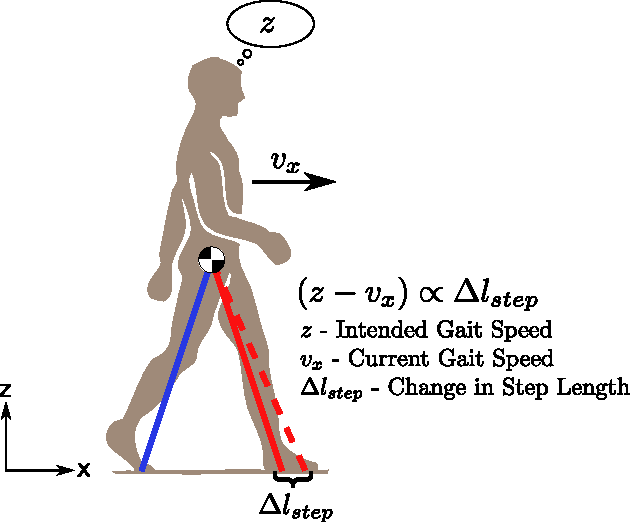
\includegraphics[width=0.5\linewidth]{main_idea}
	\caption{Change in intended velocity may be inferred from change in step length}\label{fig:main_idea}
\end{figure}

The B-SLIP model may be used to adequately model steady-state walking, and foot placement was found to be critical in optimizing periodic gaits. The model does not inherently capture the active changes required to change speed nor the first-principles humans employ for foot-placement as a function of the desired gait speed. These aspects were initially modeled by designing a controller for the B-SLIP model to emulate human motor control. With such a design, intent changes may be considered analogous to controller setpoint changes. Several theories try to explain human motor control, one of which says that the human sensorimotor system relies on optimal control \cite{todorov2004optimality,sylla2014assessing}. Therefore, we chose to assume the human motor controller to be a Linear Quadratic Regulator (LQR). The MS-to-MS Poincar\'e map was linearized about a periodic gait and the linearized model was used to design a controller that minimized deviations from a specified gait. 

The dynamics of the B-SLIP model are nonlinear and linearizing them about a single periodic gait results in a model valid for a very small portion of the gait which rendered the controller unable to handle large speed changes. A derivative-free technique i.e., the Unscented Transform \cite{manchester2016derivative} were employed to generate a linear model. This technique required integrating dynamics backward in time which was difficult to do for the hybrid dynamics of the B-SLIP model as the gait event timing cannot be fixed. Therefore, due to the lack of first principles that describe human choices to bring about intended gait changes, a data-driven approach was chosen to model the relationship between intended gait speed and foot placement.

\begin{figure}
	\centering
	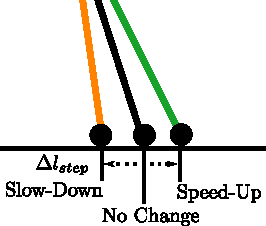
\includegraphics[width=0.35\linewidth]{step_change.pdf}
	\caption{Speed-up and slow-own increase and decrease the step length respectively}\label{fig:step_change}
\end{figure}

There is a correlation between step length and walking velocity that can be exploited to infer changes in intended gait speed. People walking at lower velocities exhibit shorter step lengths, and an increase in velocity results in an increase in step length \cite{kuo2001simple,andriacchi1977walking}, as illustrated in Fig.~\ref{fig:step_change}. Such a velocity-step-length relationship can also be viewed as valid assuming that the walk ratio is roughly constant \cite{sekiya1997optimal}. 

The walk ratio, defined as the ratio of the step length to cadence~\cite{rota2011walk}, is fairly invariant with respect to gait speeds for community ambulation, i.e.,~gait velocities greater than 0.8 m/s, despite age and terrain. It is affected when attention is divided between motor and cognitive tasks i.e., dual-task walking \cite{bogen2018walk}. The walk ratio increases as speed decreases below community ambulation velocities \cite{murakami2017estimated} and is dependent on the nature and severity of injuries \cite{rota2011walk} during unassisted walking. In rehabilitation, the variability in the walk ratio may be reduced due to the stability provided by the exoskeleton structure and consistent timing of the exoskeleton assistance \cite{seo2015new}. While the effects of exoskeleton-assisted walking on the walk ratio remain open, this analysis suggests that it is reasonable to assume a constant walk ratio for the work herein.

\section{Framework to estimate desired gait speed - Buttressed Kalman Filter}

It was assumed that intent changes made at the first MS are reflected in the placement of the foot at TD and then maintained as constant until the subsequent MS. As illustrated in Fig.~\ref{fig:step_stages}, a step starts at MS, the footstep is finalized at TD, and the step is completed at the next MS. Therefore, a twice-per-step strategy that relies on a simple model to exploit the relationship between velocity change and step length change was used to estimate intent at TD and MS. 

\begin{figure}
	\centering
	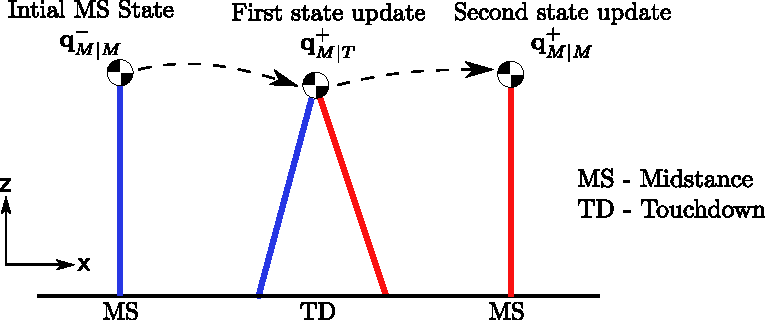
\includegraphics[width=0.75\linewidth]{step_stages.pdf}
	\caption{Two-stage estimation process}\label{fig:step_stages}
\end{figure}

A staged estimation scheme, as illustrated in Fig.~\ref{fig:block_diag}, was considered to infer intent changes using step length change information. The unit delay represents the passing of estimates as initial conditions for the next estimation cycle. In this scheme, footstep information at TD was first used to update the intent state for the initial MS. The position and velocity of the CoM were then corrected with a second update at the terminal MS of the step. A simple data-driven model of step length was used as a function of the velocity $ v_x $ at the MS prior to TD, desired velocity $ z $, and leg length $ l_{leg} $:

\begin{equation}
	l_{step} = [v_x\ (z-v_x)\ l_{leg}] \greekvec{\kappa} \label{eq:stepModel},
\end{equation}
where $ \greekvec{\kappa} $ is a vector containing regression coefficients and the model output is a scalar value in meters. This model takes into consideration the nominal step length as a function of leg length, the current velocity, and desired velocity.

\begin{figure}
	\centering
	\begin{overpic}[width=0.7\linewidth,percent]{block_diagram}
		\put(12.7,11){\scriptsize Eq.~\eqref{eq:sig_yy} - \eqref{eq:tdCovUp}}
		\put(47,11){\scriptsize Eq.~\eqref{eq:model} - \eqref{eq:P_up}}
	\end{overpic}
%	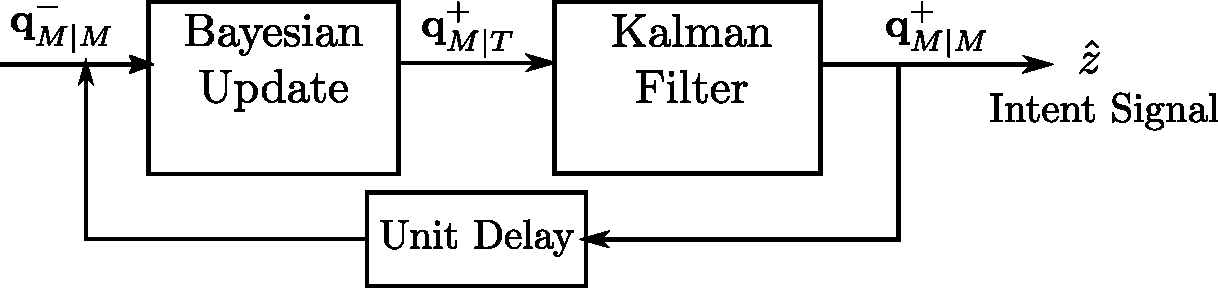
\includegraphics[width=0.7\linewidth]{block_diagram.pdf}
	\caption{Twice-per-step strategy to estimate user intent}\label{fig:block_diag}
\end{figure}

This estimation strategy is briefly  where  

The step length model may be used as a measurement model in a Kalman filter framework to relate the intended gait speed to the measured step length. The estimator operates on the the state $ \hat{\q} $ and its covariance $ \P $. In the following equations, the superscripts $ - $ and $ + $ denote pre-/post-update states respectively, the subscripts $ M $ and $ T $ denote MS and TD respectively, and the bar denotes the update location. For instance, $\hat{\q}_{M|T}^+ $ represents the state of the CoM at MS updated at TD. 

Since the footstep model is data-driven and may have inaccuracies, a process noise covariance $ \Q_{T} $ was added to the state estimate covariance $ \P^-_{M|M} $. Additionally, the estimated measurement covariance $ \Ssigma_{yy} $ was computed using the Jacobian of the measurement model $ \H_{T} $ and measurement covariance $ \R_{T} $. The predicted step length from Eq.~\eqref{eq:stepModel} was compared to the measured step length $ \tilde{\y}_{T} $. The state at MS $ \hat{\q}_{M|M}^- $ and its covariance were then updated using a Bayesian update as shown in Eq.~\eqref{eq:tdUp} and Eq.~\eqref{eq:tdCovUp}.

\begin{eqnarray}
	\hat{\y}_{T} &=&  l_{step}(\hat{v}_x,\hat{z}, l_{leg}) \nonumber \\
	\H_{T} &=& \left. \frac{\partial \hat{\y}_{T}}{\partial \q}\right|_{\hat{\q}} \nonumber \\
	\Ssigma_{yy} &=& \H_{T} \left(\P^-_{M|M} + \Q_{T}\right) \H_{T}^{\top} + \R_{T} \label{eq:sig_yy}\\
	\hat{\q}_{M|T}^+ &=& \hat{\q}_{M|M}^- + \P^- \H_{T}^{\top} \Ssigma_{yy}^{-1} (\tilde{\y}_{T} - \hat{\y}_{T})  \label{eq:tdUp}\\
	\P^+_{M|T} &=& \P^-_{M|M} -\P^-_{M|M} \H_{T}^{\top} \Ssigma_{yy}^{-1} \H_{T} \P^-_{M|M} \label{eq:tdCovUp}
\end{eqnarray}

This update to the previous MS state using TD information then primes $ \hat{\q}_{M|T}^+ $ and $ \P^+_{M|T} $ to be used with a Kalman filter.	Simple dynamics are used to propagate this state and covariance to the next MS 
\begin{eqnarray}
			\hat{\q}_{M|T}^+ &\leftarrow& \D \hat{\q}_{M|T}^+ \label{eq:model}\\
			\P^+_{M|T} &\leftarrow& \D  \P^+_{M|T} \D^{\top} + \Q_{M} \label{eq:cov}
\end{eqnarray}

These simple dynamics change the signs of the lateral position and velocity of the CoM to emulate the switching of the stance foot and allow for the application of a standard Kalman filter from MS to MS. It is assumed that the motion of the CoM is periodic with respect to the stance foot; however, since the CoM position is referenced from the stance foot, which changes step to step, the lateral position and velocity also change signs. Therefore, the propagation matrix is $ \D = {\rm diag}([1 ,-1 ,1 ,1 ,-1 ,1 ,1]) $. 

The second update takes place at the next MS, with the stance foot switched. The outputs of Eq.~\eqref{eq:model} and \eqref{eq:cov} are updated using a Kalman update 
\begin{eqnarray}
	\K &=& \P^+_{M|T} \H_{M}^{\top} \left(\H_{M} \P^+_{M|T} \H_{M}^{\top} + \R_{M}\right)^{-1}\\
	\hat{\q}_{M|M}^+ &=& \hat{\q}_{M|T}^+ + \K(\tilde{\y}_{M} - \H_{M} \hat{\q}_{M|T}^+) \\
	\P^+_{M|M} &=& (\I - \K \H_{M}) \P^+_{M|T} \label{eq:P_up}
\end{eqnarray}
where the measurement model Jacobian is $ \H_{M} = \I^{6\times7} $ since the measurements are $ \tilde{\y}_{M} = [\tilde{\p}_{CoM} ,\tilde{\v}_{CoM}]^{\top} $.

